% ----------------------------------------------------------
% Abordagem Teórica: Uma breve descrição que explique o 
% contexto teórico abordado pelo assunto.
% ----------------------------------------------------------

\chapter[Abordagem Teórica]{Abordagem Teórica}
%\addcontentsline{toc}{chapter}{Abordagem Teórica}
\section{Transistor como Chave}
	Transistor é um componente eletrônico que possui diversas aplicações na área e de muita importância em circuitos integrados, sendo uma delas a sua utilização como uma chave. 
Conforme a \autoref{figuras/fig1_BC547}, o componente possui três terminais: \textbf{emissor}, \textbf{base} e \textbf{coletor}.

\begin{figure}[htb]
\caption{\label{figuras/fig1_BC547}Representação do transistor BC547, usado em laboratório.}
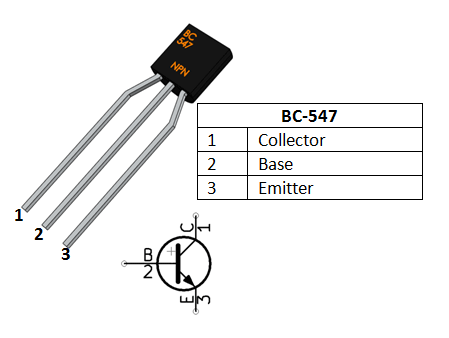
\includegraphics[scale=0.45]{figuras/fig1_BC547}
\centering
\end{figure}

	Basicamente, o coletor recebe uma tensão, o (terminal) base faz o chaveamento e emissor envia o sinal amplificado.

	O site Tecmundo\footnote{Disponível em \url{https://www.tecmundo.com.br/o-que-e/3596-o-que-e-um-transistor-e-porque-ele-e-importante-para-o-computador-.htm}} 
traz uma boa analogia sobre o funcionamento de um transitor como base onde ``(...)podemos pensar no transistor como uma torneira. O lado do cano que vem da rua é o terminal de entrada e o lado de onde sai a água 
é o terminal de saída. Quando você abre ou fecha a torneira, sua mão atua como o terminal do meio. Quanto mais você girar a 
torneira, mais água passará.''
	
\section{Corte e Saturação}

	O transistor pode trabalhar em 3 áreas de polarização: \textbf{ativa}, \textbf{corte} e \textbf{saturação}, conforme \autoref{figuras/fig2_GraficoArea}.
	Para esta experiência os pontos de corte e saturação são mais importantes. 
\begin{figure}[htb]
  \caption{\label{figuras/fig2_GraficoArea}Gráfico $I_c$ x $V_{ce}$ representando as áreas de polarização do transistor}
  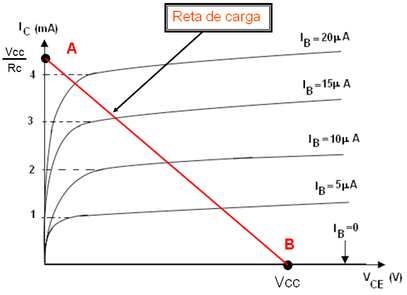
\includegraphics[scale=0.60]{figuras/fig2_GraficoArea}
  \centering
\end{figure}


A passagem da área de corte para a área de saturação é dada pela corrente aplicada na base ($I_b$). 

Quando $I_b = 0$, nosso transistor irá trabalhar na área de corte, o que significa que a corrente do coletor $I_c$ será nula. Desta forma temos: 
$$I_c = 0$$$$V_{ce} = V_{cc}$$

Já quando trabalhamos com $I_b >= I_{b_{sat}}$ o transistor operará na região de saturação onde $I_{c_{sat}} = \frac{V_{cc}}{R_c}$.
						

